%% 
%% Copyright 2007, 2008, 2009 Elsevier Ltd
%% 
%% This file is part of the 'Elsarticle Bundle'.
%% ---------------------------------------------
%% 
%% It may be distributed under the conditions of the LaTeX Project Public
%% License, either version 1.2 of this license or (at your option) any
%% later version.  The latest version of this license is in
%%    http://www.latex-project.org/lppl.txt
%% and version 1.2 or later is part of all distributions of LaTeX
%% version 1999/12/01 or later.
%% 
%% The list of all files belonging to the 'Elsarticle Bundle' is
%% given in the file `manifest.txt'.
%% 
%% Template article for Elsevier's document class `elsarticle'
%% with harvard style bibliographic references
%% SP 2008/03/01

%\documentclass[review, 12pt,authoryear]{elsarticle}
\documentclass[11 pt, onecolumn]{IEEEtran}

%% Use the option review to obtain double line spacing
%% \documentclass[authoryear,preprint,review,12pt]{elsarticle}

%% Use the options 1p,twocolumn; 3p; 3p,twocolumn; 5p; or 5p,twocolumn
%% for a journal layout:
%% \documentclass[final,1p,times,authoryear]{elsarticle}
%% \documentclass[final,1p,times,twocolumn,authoryear]{elsarticle}
%% \documentclass[final,3p,times,authoryear]{elsarticle}
%% \documentclass[final,3p,times,twocolumn,authoryear]{elsarticle}
%% \documentclass[final,5p,times,authoryear]{elsarticle}
%% \documentclass[final,5p,times,twocolumn,authoryear]{elsarticle}

%% For including figures, graphicx.sty has been loaded in
%% elsarticle.cls. If you prefer to use the old commands
%% please give \usepackage{epsfig}

%% The amssymb package provides various useful mathematical symbols
\usepackage{amssymb}
\usepackage{color}
\usepackage{graphicx}
\usepackage{amsmath}
\usepackage{wasysym}
\usepackage{multirow}
\usepackage{booktabs}
\usepackage{lineno}
\usepackage{soul}
%\usepackage{subcaption}
\usepackage[draft]{fixme}
\usepackage{longtable}
\usepackage{supertabular}
\usepackage{mathtools}
\usepackage{caption}
\usepackage{subcaption}
\usepackage{authblk}
\usepackage[colon]{natbib}
%\usepackage{hyperref}
%\hypersetup{
%	pdfpagemode = UseOutlines
%	}
%% The amsthm package provides extended theorem environments
%% \usepackage{amsthm}

%% The lineno packages adds line numbers. Start line numbering with
%% \begin{linenumbers}, end it with \end{linenumbers}. Or switch it on
%% for the whole article with \linenumbers.
%% \usepackage{lineno}


%\linenumbers

\newcommand{\delOx}{$\delta{}^{18}\mathrm{O}$ }
\newcommand{\delD}{$\delta\mathrm{D}$ }
\newcommand{\Dxs}{$\mathrm{D_{xs}}$ }
\newcommand{\delN}{$\delta{}^{15}\mathrm{N}$ }
\newcommand{\degC}{${}^{\circ}\mathrm{C}$ }

%\journal{Earth and Planetary Science Letters}

\begin{document}

%\begin{frontmatter}

%% Title, authors and addresses

%% use the tnoteref command within \title for footnotes;
%% use the tnotetext command for theassociated footnote;
%% use the fnref command within \author or \address for footnotes;
%% use the fntext command for theassociated footnote;
%% use the corref command within \author for corresponding author footnotes;
%% use the cortext command for theassociated footnote;
%% use the ead command for the email address,
%% and the form \ead[url] for the home page:
%% \title{Title\tnoteref{label1}}
%% \tnotetext[label1]{}
%% \author{Name\corref{cor1}\fnref{label2}}
%% \ead{email address}
%% \ead[url]{home page}
%% \fntext[label2]{}
%% \cortext[cor1]{}
%% \address{Address\fnref{label3}}
%% \fntext[label3]{}

\title{Supporting Online Material to the manuscript: ``An assessment of diffusion-based temperature proxies.''}

%% use optional labels to link authors explicitly to addresses:
%% \author[label1,label2]{}
%% \address[label1]{}
%% \address[label2]{}

\author[1]{C. Holme}
\author[1]{V. Gkinis}
\author[1]{B. M. Vinther}


\affil[1]{Centre for Ice and Climate, Niels Bohr Institute, University of Copenhagen, 
Juliane Maries Vej 30, DK-2100 Copenhagen, Denmark}
%\affil[2]{Institute for Alpine and Arctic Research, University of Colorado, Boulder, 1560 30th Street
%Boulder, CO 80303 USA}
%\affil[3]{Div. of Geodynamics, DTU space � National Space Institute, 
%Elektrovej, Build. 327, Kgs. Lyngby, Denmark}

\maketitle

%\begin{abstract}
%
%   	\noindent A high resolution (0.05 m) water isotopic record (\delOx) is available 
%   	from the NorthGRIP ice core. In this study we look into the water isotope 
%   	diffusion history as estimated by the spectral characteristics of the \delOx 
%   	time series covering the last 16,000 years. Based on it we infer a temperature 
%	history signal for the site.
%
%\end{abstract}


%\end{frontmatter}


%%%%%%%%%%%%%%%%%%%%%%%%%%%%%%%%%%%%%%%%%%%%%%%%%%
%%%%%%%%%%%%%%%%%%%%%%%%%%%%%%%%%%%%%%%%%%%%%%%%%%
%\tableofcontents



%%%%%%%%%%%%%%%%%%%%%%%%%%%%%%%%%%%%%%%%%%%%%%%%%%
%%%%%%%%%%%%%%%%%%%%%%%%%%%%%%%%%%%%%%%%%%%%%%%%%%
\section{Derivation of the integration equations for $\sigma^2$}


	In this section we show how we derive the numerical expressions for the diffusion length (Eq. (7) in main text).
	Starting from the differential equation for the diffusion length we have:
\begin{equation}
\frac{\mathrm{d}\sigma^2}{\mathrm{d}t} - 2\,\dot{\varepsilon}_z\!\left( t \right) \sigma^2 = 
2D\!\left( t \right).
\label{diff_len_1}
\end{equation}
	We consider the vertical strain rate due to densification:
\begin{equation}
\dot{\varepsilon}_z \left(
	t \right) = \frac{-\partial \rho}{\,\,\,\partial t}\,\frac{\,1\,}{\,\rho\,}
\label{diff_len_2}
\end{equation}
	We substitute  $t$ with $\rho$ and combine Eq.(\ref{diff_len_1}), (\ref{diff_len_2}) to get:
\begin{equation}
\frac{\mathrm{d}\sigma^2}{\mathrm{d}\rho} + \frac{2\sigma^2}{\rho} = 2 {\left(\frac{\text{d}\rho}{\text{d}t}\right)}^{-1} D(\rho)
\label{diff_len_3}
\end{equation}
	Multiplying both sides of Eq.\ref{diff_len_3} with the integrating factor 
\begin{equation}
	F(\rho) = e^{\int \frac{2}{\rho}\text{d}\rho} = \rho^2,
\label{diff_len_4}
\end{equation}
	we get:
\begin{equation}
	\frac{\text{d}}{\text{d}t} \left( \rho^2\sigma^2 \right) = 2\rho^2 {\left( \frac{\text{d}\rho}{\text{d}t} \right)}^{-1} D(\rho),
\label{diff_len_5}
\end{equation}
	from which we get the result:
\begin{equation}
\sigma^2 \left( \rho \right) = \frac{\,1\,}{\rho^2}\int_{\rho_o}^{\rho}2\rho^2 
{\left( \frac{\mathrm{d}\rho}{\mathrm{d}t}\right)}^{-1}\! D \!\left( \rho \right) \,\mathrm{d}\rho.
\label{diff_len_6}
\end{equation}

	In a similar way for the ice diffusion length (Eq. (12) in the main text) we have:
\begin{equation}
\frac{\mathrm{d}\sigma^2}{\mathrm{d}t} - 2\,\dot{\varepsilon}_z\!\left( t \right) \sigma^2 = 
2D\!\left( t \right),
\label{diff_len_7}
\end{equation}
	where the total thinning is given by:
\begin{equation}
\mathcal{S} \left( t' \right) = e^{\int_0^{t'} \dot{\varepsilon}_z \left( t \right) \mathrm{d}t} \enspace .
\label{diff_len_8}
\end{equation}
	We multiply  both sides of Eq. (\ref{diff_len_7}) with the integrating factor 
\begin{equation}
	F(\rho) = e^{\int_0^{t'}-2\dot{\varepsilon}_z \left( t \right) \mathrm{d}t},
\label{diff_len_9}
\end{equation}
	which results in
\begin{equation}
	\frac{\text{d}}{\text{d}t} \left[\sigma^2   e^{\int_0^{t'}-2\dot{\varepsilon}_z \left( t \right) \mathrm{d}t} \right] 
	= 2D(t)e^{\int_0^{t'}-2\dot{\varepsilon}_z \left( t \right) \mathrm{d}t},
\label{diff_len_10}
\end{equation}
	and gives the expression for the calculation of the ice diffusion length
\begin{equation}
\sigma_{ice}^2 \!\left( t' \right) = 
S\! \left( t' \right)^2 \,\int_0^{t'} 2 D_{ice} \!\left( t \right) S \!\left( t \right) ^{-2} \,\mathrm{d} t.
\label{diff_len_11}
\end{equation}
	
%%%%%%%%%%%%%%%%%%%%%%%%%%%%%%%%%%%%%%%%%%%%%%%%%%
%%%%%%%%%%%%%%%%%%%%%%%%%%%%%%%%%%%%%%%%%%%%%%%%%%


\section{The diffusivity parametrization} \label{D_appendix}
\subsection{The firn diffusivity}
We used the diffusivity parametrization as introduced by \cite{Johnsen2000}.
\begin{equation}
D \!\left(\rho\right) = \frac{m\,p\,D_{ai}}{R\,T\,\alpha_i\,\tau}
\left(\frac{\,1\,}{\,\rho\,} - \frac{\,1\,}{\,\rho_{ice}\,}\right).
\label{eq2.8}
\end{equation}
	The terms used in Eq. (\ref{eq2.8}) and their parameterizations used are described below: 
\begin{itemize}

\item{$m$ is the molar weight (kg)}

\item{$p$: saturation vapor pressure over ice (Pa). We use \cite{Murphy2005}:
\begin{equation}
p = \exp \left(9.5504 - \frac{5723.265}{T} + 3.530\,\ln\!\left( T \right) - 0.0073\,T \right).
\label{eq2.9}
\end{equation}}

\item{$D_{a}$:  diffusivity of water vapor in air ($\mathrm{m}^2 \mathrm{s}^{-1}$). We use \citep{Hall1976}:
\begin{equation}
D_{a} = 2.1\cdot 10^{-5} {\left(\frac{T}{T_o}\right)}^{1.94} \left(\frac{P_o}{P}\right)
\label{eq2.10}
\end{equation}
with $P_o = 1$ Atm, $T_o = 273.15$ K and $P, \;T$ the ambient pressure (Atm) and temperature (K).
Additionally from \cite{Merlivat1979} $D_{a^2\mathrm{H}} = \frac{D_a}{1.0285}$ and 
$D_{a^{18}\mathrm{O}} = \frac{D_a}{1.0251}$}.

\item{$R$: molar gas constant $R = 8.314478 \,\,\left(\mathrm{m}^3\mathrm{Pa}\,\left(\mathrm{K \,mol}\right)^{-1}\right)$}

\item{$T$: Ambient temperature (K)}

\item{$\alpha_i$: Ice -- Vapor fractionation factor.  we use the formulations by \cite{Majoube1971} 
and \cite{Merlivat1967} for $\alpha_{s/v}^{2}$ and $\alpha_{s/v}^{18}$ respectively.
\begin{align}
\ln \alpha_{Ice/Vapor} \left(^{2}\mathrm{H}/^{1} \mathrm{H} \right) &= 16288/T^2 - 9.34 \times 10^{-2}\\
\ln \alpha_{Ice/Vapor} \left( ^{18}\mathrm{O}/^{16} \mathrm{O} \right) &= 11.839/T - 28.224 \times 10^{-3}
\label{eq2.12}
\end{align}}

\item{$\tau$: The firn tortuosity. We use \citep{Schwander1988, Johnsen2000}:
\begin{equation}\label{eq2.13}
\frac{1}{\tau } = 
\left\{ 
  \begin {array}{ll}
1 - b_\tau  \left( {\frac{\rho }{{\rho _{ice} }}} \right)^2 & \mbox{, for } \rho  \le \frac{\rho_{ice}}{\sqrt{b}}  \\
0 & \mbox{, for } \rho  > \frac{\rho_{ice}}{\sqrt{b}}\\
 \end{array}\right. \enspace,
\end{equation}
	where $b_\tau = 1.30$, implying a close-off density of $\rho_{\mathrm{co}} = 804.3\;\mathrm{kgm}^{-3}$.}

\end{itemize}

\subsection{The ice diffusivity}
	Ice diffusion  is believed to occur via a vacancy mechanism 
	with transport of molecules within the ice lattice.
	Based on isotopic probe experiments, there is a strong consensus that 
	the ice diffusivity coefficient is  the same for 
	$\mathrm{H}_2 \,^{18}\mathrm{O}, \, \mathrm{D}_2 \mathrm{O} \text{ and } \mathrm{T}_2 \mathrm{O}$
	\citep{Ramseier1967, Blicks1966, Itagaki1967, Delibaltas1966}
	The dependence of the ice diffusivity parameter to temperature is described by
	an Arrhenius type equation
\begin{equation}
D = D_0 \exp \left( -Q/RT \right),
\label{arrhenius}
\end{equation}
	where $Q$ is the activation energy and $D_0$ a pre-exponential factor.
	The results of the studies mentioned above agree well with each other and here we
	plot the diffusivity parametrization coefficients suggested by those studies (Fig. \ref{ice_diffusivities_plot}). 
	The ice diffusion length calculations in our work use the results of \cite{Ramseier1967} 
	according to which we use $Q = 0.62 \; \mathrm{eV}$ and $D_{o} = 9.2\cdot10^{-4}  \; \mathrm{m^2\,s^{-1}}$.
	Note that the results of \cite{Ramseier1967} are based on measurements of both artificially as well
	as naturally grown ice   collected at Mendenhall glacier, Alaska.

%%%%%%%%%%%%%%%%%%%%%%%%%%%%%%%%%%%%%%%%%%%%%%%%%%
%%%%%%%%%%%%%%%%%%%%%%%%%%%%%%%%%%%%%%%%%%%%%%%%%%
\section{Examples of diffusion lengths for different ice core sites}
	In this section we present an ensemble of implementations of the diffusion--densification model  
	for various combinations of surface forcings that represent typical modern day conditions
	for a number of ice core sites on Greenland and Antarctica.
	The contours in the plot are generated by integration of Eq. (\ref{diff_len_6}) and expressed
	in m ice eq.
	The forcing for each ice core site is given in Table \ref{sigma_18_core_sites} and the 
	results are shown in Fig. \ref{diffusionlength_map}.



%%%%%%%%%%%%%%%%%%%%%%%%%%%%%%%%%%%%%%%%%%%%%%%%%%
%%%%%%%%%%%%%%%%%%%%%%%%%%%%%%%%%%%%%%%%%%%%%%%%%%
\section{Estimation of $\sigma^2$ from the high resolution data set}
	
	In order to estimate the diffusion length value from high resolution water isotope data we minimize the 
	2-norm $\| P_s - \hat{P}_s \|$ where $\hat{P}_s$ is an estimate of the power spectral density of 
	a high resolution \delOx data section and $P_s$ is a model description of the power spectral density.
	
	The estimate of the power spectral density $\hat{P}_s$ of a \delOx dataset is obtained by the use
	of the Burg's spectral estimation method. The method fits an autoregressive model 
	of order $\mu$ (AR-$\mu$) by minimizing the forward--backward prediction error filter 
	\citep{Hayes1996, RECIPES, Andersen1974}.
	For the theoretical model  we have:
\begin{equation}
\label{powersd}
P_s =  P_{\sigma}  + {\vert \hat{\eta} \left( k \right) \vert} ^{2},
\end{equation}%e11
	where $P_{\sigma} = P_0 \,{e}^{-k^2 \sigma_i^2}$ is the effect of the 
	firn diffusion process with diffusion length $\sigma^2$.
	Regarding the noise, we find red noise described by an AR-1 process with an autoregressive coefficient
	$q_1 = 0.15$ to provide a 
	good description of the noise signal we observe. The spectrum of
	this signal is of the form \citep{Kay1981}:
\begin{equation}
|\hat{\eta}(k )|^2 = \frac{\sigma_{\eta}^2 \Delta} {\left| 1+q_1 \exp{\left( - i k \Delta \right) } \right|^2} {},
\label{rednoise}
\end{equation}%e21
 	where $\sigma_{\eta}^2$ is the variance of the noise.
	The angular frequency $k=2\pi f$  is in the range $f \in \left[ 0, \; \frac{1}{2\Delta}  \right] $
	defined by the Nyquist frequency and thus the sampling resolution $\Delta$.
	We vary the parameters
	$\sigma^2, \, P_0, $ and $\sigma_{\eta}^2$ of the spectral model 
	in order to minimize the misfit
	between $P_s$ and  $\hat{P}_s$ in the least squares sense.
	
	As it can be  seen in  Fig.\ref{spectral01}, it is the characterization of the spectrum as a whole that yields
	information on $\sigma^2$. It is thus not necessary to specifically study the relative attenuation 
	of individual spectral peaks as for example the annual signal. This approach allows for a study 
	of the diffusion signal even after the spectral signature of the annual signal diminishes below
	detection limit. 
	

	
\subsection{AR order selection}
\label{AR_order_selection}
	An interesting feature of the Burg estimation method is that 
	the order $\mu$ of the AR filter affects the spectral resolution of the spectral estimate \citep{Hayes1996, RECIPES}. 
	Low $\mu$
	values result in smoother spectra with inferior spectral resolution, while higher order spectra show better
	performance in resolving neighboring spectral peaks. This can be seen in the spectral estimates
	presented in Fig.\ref{spectral01} where we plot spectral estimates with  $\mu = 30$ and 
	$\mu = 40$.
	As described above, the goal of the $\sigma^2$ estimation is to characterize the overall shape of the spectrum. 
	As a result, relatively low values of $\mu$
	produce smooth spectra of relatively low spectral resolution and can be
	adequate for the purpose of our application.
	
	We look into both the influence of the $\mu$ value on the $\sigma^2$ estimate
	by performing 41 power spectrum estimates with $\mu \in \left[ 40, 80 \right]$.  
	Possible interferences of spectral features due to longer scale climate variability that could have
	an effect on the estimation of $\sigma^2$ are also investigated with this test.
	In Fig.\ref{spectral02} we show the mean value
	of the 41 spectral estimates before and after strain correction. 
	The standard deviation of the estimated
	$\sigma^2$ for every depth is presented on the top subplot of the figure. 
	It can be seen that on average
	the standard deviation is about 2 orders of magnitude lower than the absolute values of $\sqrt{\sigma^2}$
	thus  approximately in the 1\% range.  
	The low standard deviation of the 41 estimates suggests that a possible 
	effect of spectral features due to low frequency climate variability is of second order. 
	It also indicates
	that the selection of the AR order $\mu$, in Burg's spectral estimation is 
	not a critical aspect of the estimation process.
	


\subsection{Ice flow effects on the spectral estimation}
	With depth increasing and due to the ice flow thinning, 
	every discrete ice core sample cut at resolution $\Delta$ will represent an increasing number of years. 
	This should not have an effect on the estimate of $\sigma^2$. 
	As seen in Eq. (4) and  of the 
	MT, the diffusion process is seen as the convolution of the initial $\delta$ profile with a Gaussian filter.
	The convolution operation takes place in the $z$ domain. 
	It conclusively follows  that the transfer
	function of the diffusion process is a function  of $k = 2\pi/\Delta$ and as a result estimation 
	of $\sigma^2$ is performed using the power spectrum in the $k$ domain. 
	
	For the same reason,
	the correction term $\sigma_{dis}^2$, used in order to account for the diffusion imposed by the
	discrete sampling scheme is also a parameter that is constant with depth.
	Due to the ice layer thinning, percentage wise, 
	the discrete sampling correction increases with depth. It is also evident that
	with a constant value, $\sigma_{dis}^2$ represents an increasing number of years for higher depths.
	In Fig. \ref{discrete_sampling01}, 
	we illustrate the effect of this correction. 

	
	At increasing depths, $\sigma^2$  will be decreasing due to ice flow thinning. 
	At lower $\sigma^2$ values, a spectrum estimate up to the 
	Nyquist frequency $1/2\Delta$ will contain a decreasing
	part of the noise signal  ${\vert \hat{\eta} \left( k \right) \vert} ^{2}$. After a certain depth, 
	the sampling resolution is not high enough to resolve the noise signal. The result of 
	this effect is that the estimation of the $P_{\sigma}$ signal requires  an
	assumption about ${\vert \hat{\eta} \left( k \right) \vert} ^{2}$
	and thus can limit  the  extend to which the diffusion technique can be 
	applied to the deeper parts of the core. 
	
	In Fig. \ref{spectral04} we plot the expected diffusion length value assuming a simple case of constant temperature 
	and accumulation rate at the surface and a certain ice layer thinning history. 
	Then, based on this modeled
	diffusion length profile, in Fig. \ref{spectral03}, we create a series of six power spectral densities for 
	$z = 200, 600, 900, 1200, 1400 \, \mathrm{ and } \, 1600  \, \mathrm{m}$. 
	The spectral models are calculated
	using 2 different sampling schemes, $\Delta_1 = 5 \, \mathrm{cm \; and \;} \Delta_2 = 2.5 \,\mathrm{cm}$.
	The plots illustrate the effect of the ice layer thinning as well as the sampling resolution
	on the shape of the power spectral density. 
	As depth increases, a progressively smaller portion of the noise signal is resolved. 
	Conclusively, for the deeper parts of the core where the ice layer thinning 
	has reduced the diffusion length, a higher sampling resolution ($\Delta < 2.5 \, \mathrm{cm}$) 
	is preferable  for an accurate estimation of $P_s$ and subsequently $\sigma^2$ to be possible. 
	For the NorthGRIP reconstruction we present here, we are able resolve the noise signal down to the
	depth of approximately 1450 m. 
	For depths higher than 1450 m we make the simplest possible assumption that the noise level
	is equal to the average values we have observed in the Holocene section. 
	





%%%%%%%%%%%%%%%%%%%%%%%%%%%%%%%%%%%%%%%%%%%%%%%%%%
%%%%%%%%%%%%%%%%%%%%%%%%%%%%%%%%%%%%%%%%%%%%%%%%%%

\section{Estimation of the uncertainties involved}
	
	In this section we assess the uncertainties involved in the estimation of the
	temperature.
	We identify two main sources of uncertainty. Those related to the parameters
	of the firn densification model and those related to the ice flow thinning.
	Each of these two sources of uncertainty is involved at  different stages of the calculation
	and affect the estimation of the temperature in  different ways. 
	
	Uncertainties related to the firn densification model have an impact on the
	inferred variability of the temperature signal. Centennial to millennial scale temperature 
	signals as well as the amplitudes of climatic transitions will be affected by this type of uncertainty.
	On the contrary, the uncertainty associated with
	the ice thinning correction  affects the slope of the signal.  Relatively small variations
	in the thinning function can result in differences of several degrees in temperature.
	However this type of uncertainty can be minimized if estimates of temperature 
	based on other proxies are available and can be used as tie points. In this case 
	the firn diffusion technique can provide combined information on both the temperature history 
	and the ice flow characteristics of the ice core site. 
	
	
\subsection{Firn densification model}
	
	Uncertainties related to the densification model affect the estimation of the diffusion 
	length  $\sigma^2_{\mathrm{firn}}$ at the close--off depth. Hereby we examine the 
	influence of four parameters involved in the densification--diffusion model. We run
	a set of sensitivity experiments where the four firn densification parameters 
	are perturbed in order to create a family of 1000 implementations of the diffusion-densification
	model for each experiment. For all the following sensitivity tests we also consider
	the standard deviation of the diffusion length spectral estimate as calculated in 
	section  \ref{AR_order_selection}.
	
	The first two parameters we consider are the surface and close--off densities $\rho_0$ and $\rho_{\mathrm{co}}$. 
	We perform two sensitivity experiments where  the values of
	$\rho_0$ and $\rho_{\mathrm{co}}$ are drawn from  a Gaussian distribution with a 
	defined mean and standard deviation (Table \ref{table_mctests}). 
	For the close--off density
	a value of $804 \;  \pm 20 \;\text{kgm}^{-3} \;(1\sigma)$ is used  
	\citep{Schwander1988, Jean-Baptiste1998, Johnsen2000}.
	The range of values we choose for $\rho_\text{co}$ brackets within $2\sigma$ the more 
	extreme estimates of $775 \; \text{and} \; 840  \;\text{kgm}^{-3}$ shown in
	\cite{Scher1970} and \cite{Stauffer1985} respectively.
	For the surface density we use a  value of 
	$320 \pm 40 \;\text{kgm}^{-3} \;(1\sigma)$, based on modern observations of
	the firn column density at NothGRIP. Previous high resolution density observations by
	\cite{Albert2002} for Summit, Greenland indicate that the surface density can 
	vary within $\pm 50 \mathrm{kgm}^{-3}$ of its mean value and as a result a $1\sigma$
	of $ 40 \;\mathrm{kgm}^{-3}$ assures that the Gaussian distribution of $\rho_0$
	covers this range adequately in our sensitivity experiments.
	
	We also include two parameters that describe the dependance 
	of the densification rate to temperature. Based on \cite{Herron1980} 
\begin{equation}
\frac{\mathrm{d}\rho(z)}{\mathrm{d}t} = K(T)A^{\vartheta} \frac{\rho_{\mathrm{ice}} - \rho(z)}{\rho_{\mathrm{ice}}},
\label{eqhl}
\end{equation}
	where $K(T)$ is a temperature dependent Arrhenius--type densification rate coefficient described by:
\begin{equation}
K(T) = 11 \exp \left( - \frac{10160}{RT} \right)\;\;\; \rho<550 \; \mathrm{kgm}^{-3},
\label{ko_herron}
\end{equation}
and
\begin{equation}
K(T) = 575 \exp \left( - \frac{21400}{RT} \right) \;\;\; \rho\ge 550 \; \mathrm{kgm}^{-3}.
\label{k1_herron}
\end{equation}
	In order to perturb the model we  use the term $K'(t)$ in Eq. (\ref{eqhl}) where
	$K'(T) = fK(T)$ and $f = 1 \pm 0.2 \; (1\sigma)$. This results in a family of density profiles that are used 
	for the diffusion length calculation. In Fig. \ref{density_NGRIP_fof1} $1\sigma$
	and $2\sigma$ intervals are illustrated together with firn density measurements from 
	NorthGRIP.
	

 
 
	The results of these sensitivity experiments are illustrated in Fig.\ref{mc_tests_results}.
	Based on these results we conclude that using
	a fixed value for the surface and close--off densities is a plausible approach. The combined uncertainty 
	of the $\rho_o$ and $\rho_{\text{co}}$ parameters is in the order of 1 K and thus 
	the temperature history we infer is consistent over a wide range of densification parameter
	values.
	

	
\subsection{Ice flow thinning uncertainties}
	Uncertainties related to ice flow thinning depend on the accuracy of 
	the ice flow model in inferring the ice thinning function.
	The value of the diffusion length of a layer at depth $z$, estimated from the spectral properties of
	a set of \delOx data needs to be corrected for ice flow thinning.
	An incorrectly estimated  thinning function
	affects the inferred values of the diffusion length $\sigma^2_\text{firn}$ in a linear
	way as we show in Eq. (13) and (20) of the main text. As far as the inferred temperatures
	are concerned,  the ice thinning function impacts the slope of the signal, thus 
	presenting an increasing error with depth.  
	
	In Fig. \ref{strain_uncertainty} we performed the temperature calculation using six different
	scenarios for the ice thinning function $S(z)$. We assume the simple scenario of 
	thinning function that varies linearly 
	with depth and a value of $S(z = 2100 \;\text{m})$ equal to  $0.22, 0.24, 0.26, 0.28, 0.30, 0.32$. 
	It is apparent that the change in temperature due to thinning function differences is significant. 
	However the nature of this type of uncertainty, affecting only the slope of the signal, is such
	that unrealistic thinning function scenarios are relatively easy to disregard. Previous,
	estimates of temperature for any point in the climatic history of the record, 
	obtained by other proxies, can be useful  as they can help selecting a plausible 
	scenario for the thinning function and thus fix the slope of the temperature signal inferred
	with the use of the firn diffusion method.
	
	This characteristic, points to the usefulness of the method in providing combined 
	paleotemperature and glaciological information. In this study the unrealistically high
	temperature values we inferred for the Holocene climatic optimum pointed to possible
	inaccuracies of the ice thinning function used for the estimation.
	When fixing the temperature gradient
	between the Holocene optimum and present conditions to be approximately 3 K,
	as inferred from previous studies \citep{DahlJensen1998, Johnsen1995a, Johnsen2001}
	we were able to propose a more likely scenario for the ice thinning function and as a result 
	the accumulation rate history. The temperature reconstruction using the proposed ice thinning
	function is presented in red color in Fig. \ref{strain_uncertainty}.
	


	
%
%%%%%%%%%%%%%%%%%%%%%%%%%%%%%%%%%%%%%%%%%%%%
%%%%%%%%%%%%%%%%%%%%%%%%%%%%%%%%%%%%%%%%%%%

%% If you have bibdatabase file and want bibtex to generate the
%% bibitems, please use
%%
%\bibliographystyle{elsarticle-harv} 
%\bibliography{/Users/vasilis/Documents/ref's/bib_vasi.bib}

%% else use the following coding to input the bibitems directly in the
%% TeX file.
%% If you have bibdatabase file and want bibtex to generate the
%% bibitems, please use
%%
\bibliographystyle{harvard} 
%\bibliography{BitexLib.bib}
%\bibliography{/Users/vasilis/Documents/ref's/bib_vasi.bib}
%% else use the following coding to input the bibitems directly in the
%% TeX file.


\begin{thebibliography}{23}
%\expandafter\ifx\csname natexlab\endcsname\relax\def\natexlab#1{#1}\fi
%\expandafter\ifx\csname url\endcsname\relax
%  \def\url#1{\texttt{#1}}\fi
%\expandafter\ifx\csname urlprefix\endcsname\relax\def\urlprefix{URL }\fi

\bibitem[{Albert and Shultz(2002)}]{Albert2002}
Albert, M.~R., Shultz, E.~F., May 2002. Snow and firn properties and air-snow
  transport processes at summit, greenland. Atmospheric Environment 36~(15-16),
  2789--2797.

\bibitem[{Andersen(1974)}]{Andersen1974}
Andersen, N., 1974. Calculation of filter coefficients for maximum entropy
  spectral analysis. Geophysics 39~(1), 69--72.

\bibitem[{Blicks et~al.(1966)Blicks, Dengel, and Riehl}]{Blicks1966}
Blicks, H., Dengel, O., Riehl, N., 1966. Diffusion von protonen (tritonen) in
  reinen und dotierten eis-einkristallen. Physik Der Kondensiterten Materie
  4~(5), 375--381.

\bibitem[{Dahl~Jensen et~al.(1998)Dahl~Jensen, Mosegaard, Gundestrup, Clow,
  Johnsen, Hansen, and Balling}]{DahlJensen1998}
Dahl~Jensen, D., Mosegaard, K., Gundestrup, N., Clow, G.~D., Johnsen, S.~J.,
  Hansen, A.~W., Balling, N., Oct. 1998. Past temperatures directly from the
  greenland ice sheet. Science 282~(5387), 268--271.

\bibitem[{Delibaltas et~al.(1966)Delibaltas, Dengel, Helmreich, Riehl, and
  Simon}]{Delibaltas1966}
Delibaltas, P., Dengel, O., Helmreich, D., Riehl, N., Simon, H., 1966.
  Diffusion von $^{18}\text{O}$ in eis-einkristallen. Physik Der Kondensiterten
  Materie 5~(3), 166--170.

\bibitem[{Hall and Pruppacher(1976)}]{Hall1976}
Hall, W.~D., Pruppacher, H.~R., 1976. Survival of ice particles falling from
  cirrus clouds in subsaturated air. Journal of the Atmospheric Sciences
  33~(10), 1995--2006.

\bibitem[{Hayes(1996)}]{Hayes1996}
Hayes, M.~H., 1996. Statistical digital signal processing and modeling. John
  Wiley \& Sons.

\bibitem[{Herron and Langway(1980)}]{Herron1980}
Herron, M.~M., Langway, C.~C., 1980. Firn densification - an empirical-model.
  Journal Of Glaciology 25~(93), 373--385.

\bibitem[{Itagaki(1967)}]{Itagaki1967}
Itagaki, K., Feb. 1967. Self-diffusion in single crystal ice. J. Phys. Soc.
  Jpn. 22~(2), 427--431.

\bibitem[{Jean-Baptiste et~al.(1998)Jean-Baptiste, Jouzel, Stievenard, and
  Ciais}]{Jean-Baptiste1998}
Jean-Baptiste, P., Jouzel, J., Stievenard, M., Ciais, P., May 1998.
  Experimental determination of the diffusion rate of deuterated water vapor in
  ice and application to the stable isotopes smoothing of ice cores. Earth And
  Planetary Science Letters 158~(1-2), 81--90.

\bibitem[{Johnsen et~al.(2000)Johnsen, Clausen, Cuffey, Hoffmann, Schwander,
  and Creyts}]{Johnsen2000}
Johnsen, S.~J., Clausen, H.~B., Cuffey, K.~M., Hoffmann, G., Schwander, J.,
  Creyts, T., 2000. Diffusion of stable isotopes in polar firn and ice. the
  isotope effect in firn diffusion. In: Hondoh, T. (Ed.), Physics of Ice Core
  Records. Hokkaido University Press, Sapporo, pp. 121--140.

\bibitem[{Johnsen et~al.(1995)Johnsen, Dahl~Jensen, Dansgaard, and
  Gundestrup}]{Johnsen1995a}
Johnsen, S.~J., Dahl~Jensen, D., Dansgaard, W., Gundestrup, N., Nov. 1995.
  Greenland paleotemperatures derived from grip bore hole temperature and ice
  core isotope profiles. Tellus Series B-Chemical And Physical Meteorology
  47~(5), 624--629.

\bibitem[{Johnsen et~al.(2001)Johnsen, DahlJensen, Gundestrup, Steffensen,
  Clausen, Miller, Masson-Delmotte, Sveinbjornsdottir, and White}]{Johnsen2001}
Johnsen, S.~J., DahlJensen, D., Gundestrup, N., Steffensen, J.~P., Clausen,
  H.~B., Miller, H., Masson-Delmotte, V., Sveinbjornsdottir, A.~E., White, J.,
  2001. Oxygen isotope and palaeotemperature records from six Greenland
  ice-core stations: Camp Century, Dye-3, GRIP, GISP2, Renland and NorthGrip.
  Journal Of Quaternary Science 16~(4), 299--307.

\bibitem[{Kay and Marple(1981)}]{Kay1981}
Kay, S.~M., Marple, S.~L., 1981. Spectrum analysis - a modern perspective.
  Proceedings Of The Ieee 69~(11), 1380--1419.

\bibitem[{Majoube(1971)}]{Majoube1971}
Majoube, M., 1971. Fractionation in O-18 between ice and water vapor. Journal
  De Chemie Physique Et De Physico-Chimie Biologique 68~(4), 625--\&.

\bibitem[{Merlivat and Jouzel(1979)}]{Merlivat1979}
Merlivat, L., Jouzel, J., 1979. Global climatic interpretation of the
  deuterium-oxygen 18 relationship for precipitation. J. Geophys. Res. 84(C8),
  5029--5033.

\bibitem[{Merlivat and Nief(1967)}]{Merlivat1967}
Merlivat, L., Nief, G., 1967. Fractionnement isotopique lors des changements
  detat solide-vapeur et liquide-vapeur de leau a des temperatures inferieures
  a 0 degrees c. Tellus 19~(1), 122--127.

\bibitem[{Murphy and Koop(2005)}]{Murphy2005}
Murphy, D.~M., Koop, T., Apr. 2005. Review of the vapour pressures of ice and
  supercooled water for atmospheric applications. Quarterly Journal Of The
  Royal Meteorological Society 131~(608), 1539--1565.

\bibitem[{Press et~al.(2007)Press, Teukolsky, Vetterling, and
  Flannery}]{RECIPES}
Press, W.~H., Teukolsky, S.~A., Vetterling, W.~T., Flannery, B.~P., August
  2007. Numerical Recipes: The Art of Scientific Computing. {Cambridge
  University Press}.

\bibitem[{Ramseier(1967)}]{Ramseier1967}
Ramseier, R.~O., 1967. Self-diffusion of tritium in natural and synthetic ice
  monocrystals. Journal Of Applied Physics 38~(6), 2553--2556.

\bibitem[{Scher and Zallen(1970)}]{Scher1970}
Scher, H., Zallen, R., 1970. Critical density in percolation processes. Journal
  of Chemical Physics 53~(9), 3759--3761.

\bibitem[{Schwander et~al.(1988)Schwander, Stauffer, and Sigg}]{Schwander1988}
Schwander, J., Stauffer, B., Sigg, A., 1988. Air mixing in firn and the age of
  air at pore close-off. Annals Of Glaciology 10, 141--145.

\bibitem[{Stauffer et~al.(1985)Stauffer, Schwander, and H.}]{Stauffer1985}
Stauffer, B., Schwander, J., H., O., 1985. Enclosure of air during
  metamorphosis of dry firn to ice. Annals of Glaciology 6, 108--112.


\end{thebibliography}

\newpage

\begin{table}	
\begin{tabular}{l | l r r r}
Site & Location & Accum. Rate $[\text{myr}^1]$ & Temperature [C] & $\sigma_{18}^2$ [m]  \\\hline
Dome C & $75^{\circ}06'\text{S}\; 123^{\circ}21'\text{E}$ & 0.027 &  -54.5 & 0.067\\
GISP2 & $72^{\circ}36'\text{N}\; 38^{\circ}30'\text{W}$ & 0.24 & -31.4 & 0.079\\
GRIP & $72^{\circ}35'\text{N}\; 37^{\circ}38'\text{W}$ & 0.23 & -31.7 & 0.0795\\
NEEM & $77^{\circ}45'\text{S}\; 51^{\circ}06'\text{W}$ & 0.2 & -30 & 0.088\\
NorthGRIP & $75^{\circ}10'\text{N}\; 42^{\circ}32'\text{W}$ & 0.207 & -32 & 0.081\\
SipleDome & $81^{\circ}40'\text{S}\; 148^{\circ}46'\text{W}$ & 0.087 & -25 & 0.145\\
South Pole & $90^{\circ}\text{S}\; 00^{\circ}$ & 0.076 & -51 & 0.054\\
Vostoc & $78^{\circ}27'\text{S}\; 10^{\circ}51'\text{E}$ & 0.024 & -55.5 & 0.067\\
\hline
\end{tabular}
\caption{Surface forcing used for the diffusion length calculations in Fig. \ref{diffusionlength_map}. }
\label{sigma_18_core_sites}
\end{table}

\begin{table}	
\begin{tabular}{l | c c c r r}
 & $f_o$ & $f_1$ & $\rho_0$ & $\rho_\text{co}$ \\ \hline
Experiment 1 & 1 & 1 & 320 $\text{kgm}^{-3}$ & $804 \pm 20 \text{kgm}^{-3}$ \\
Experiment 2 & 1 & 1 & $320 \pm 40 \; \text{kgm}^{-3}$ & $804 \; \text{kgm}^{-3}$ \\
Experiment 3 & $1 \pm 0.2$ & $1 \pm 0.2$ & 320 \;$\text{kgm}^{-3}$ & $804 \;\text{kgm}^{-3}$ \\
Experiment 4 & $1 \pm 0.2$ & $1 \pm 0.2$ & $320 \pm 40 \; \text{kgm}^{-3}$ & $804 \pm 20 \;\text{kgm}^{-3}$ \\
\hline
\end{tabular}
\caption{Summary of the sensitivity experiments run}
\label{table_mctests}
\end{table}

\newpage


\begin{figure}
\vspace*{1mm}
\center
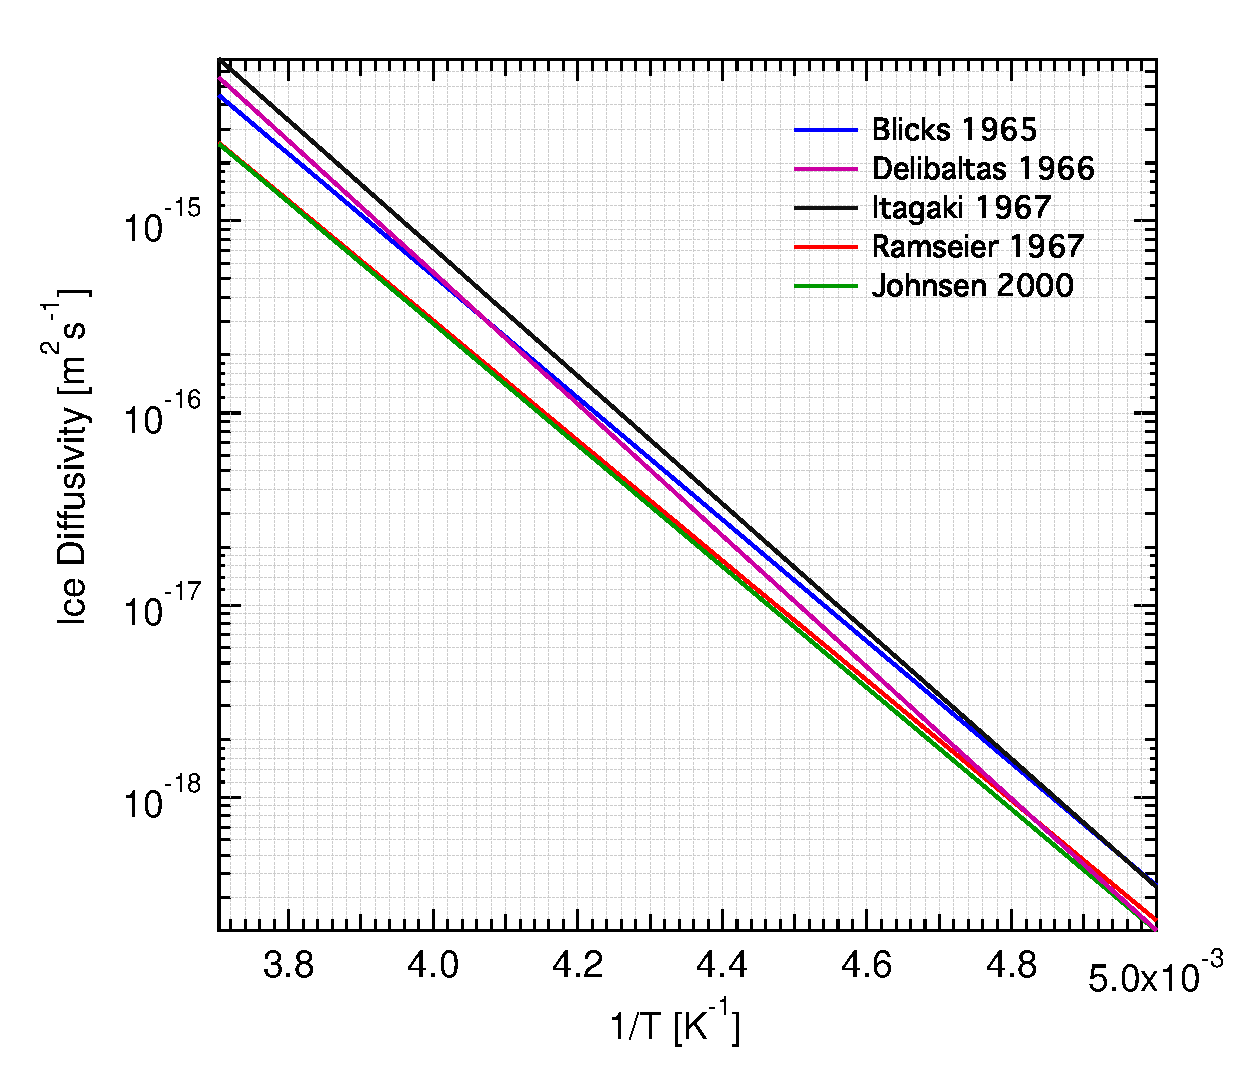
\includegraphics[width = 100mm]{./ice_diffusion}
\caption{Ice diffusivity parametrizations based on isotopic probe experiments 
for the temperature range 200 -- 270 K}
\label{ice_diffusivities_plot}
\end{figure}

\begin{figure}
\vspace*{1mm}
\center
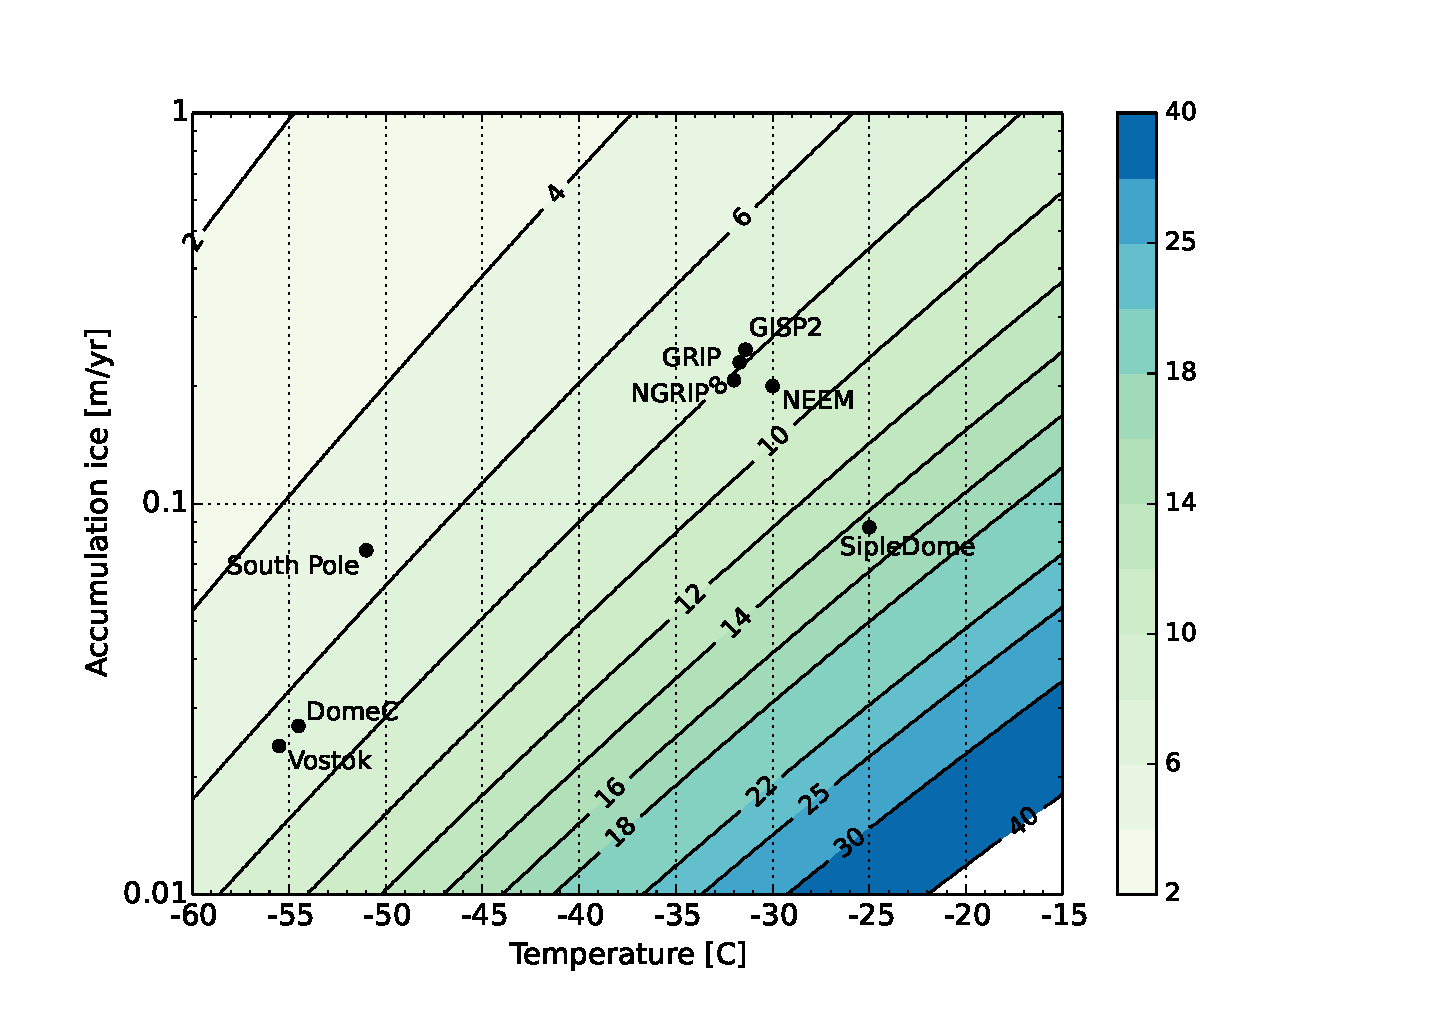
\includegraphics[width = 180mm]{./diffusionlength_map}
\caption{Calculation of $\sigma_{18}^2$ for the close--off density of $\rho_{\text{co}} = 804.3\;\text{kgm}^{-3}$ in 
m of ice equivalent. We used the same surface density $\rho_o = 330\;\text{kgm}^{-3}$ for all sites.}
\label{diffusionlength_map}
\end{figure}

\begin{figure}
\vspace*{1mm}
\center
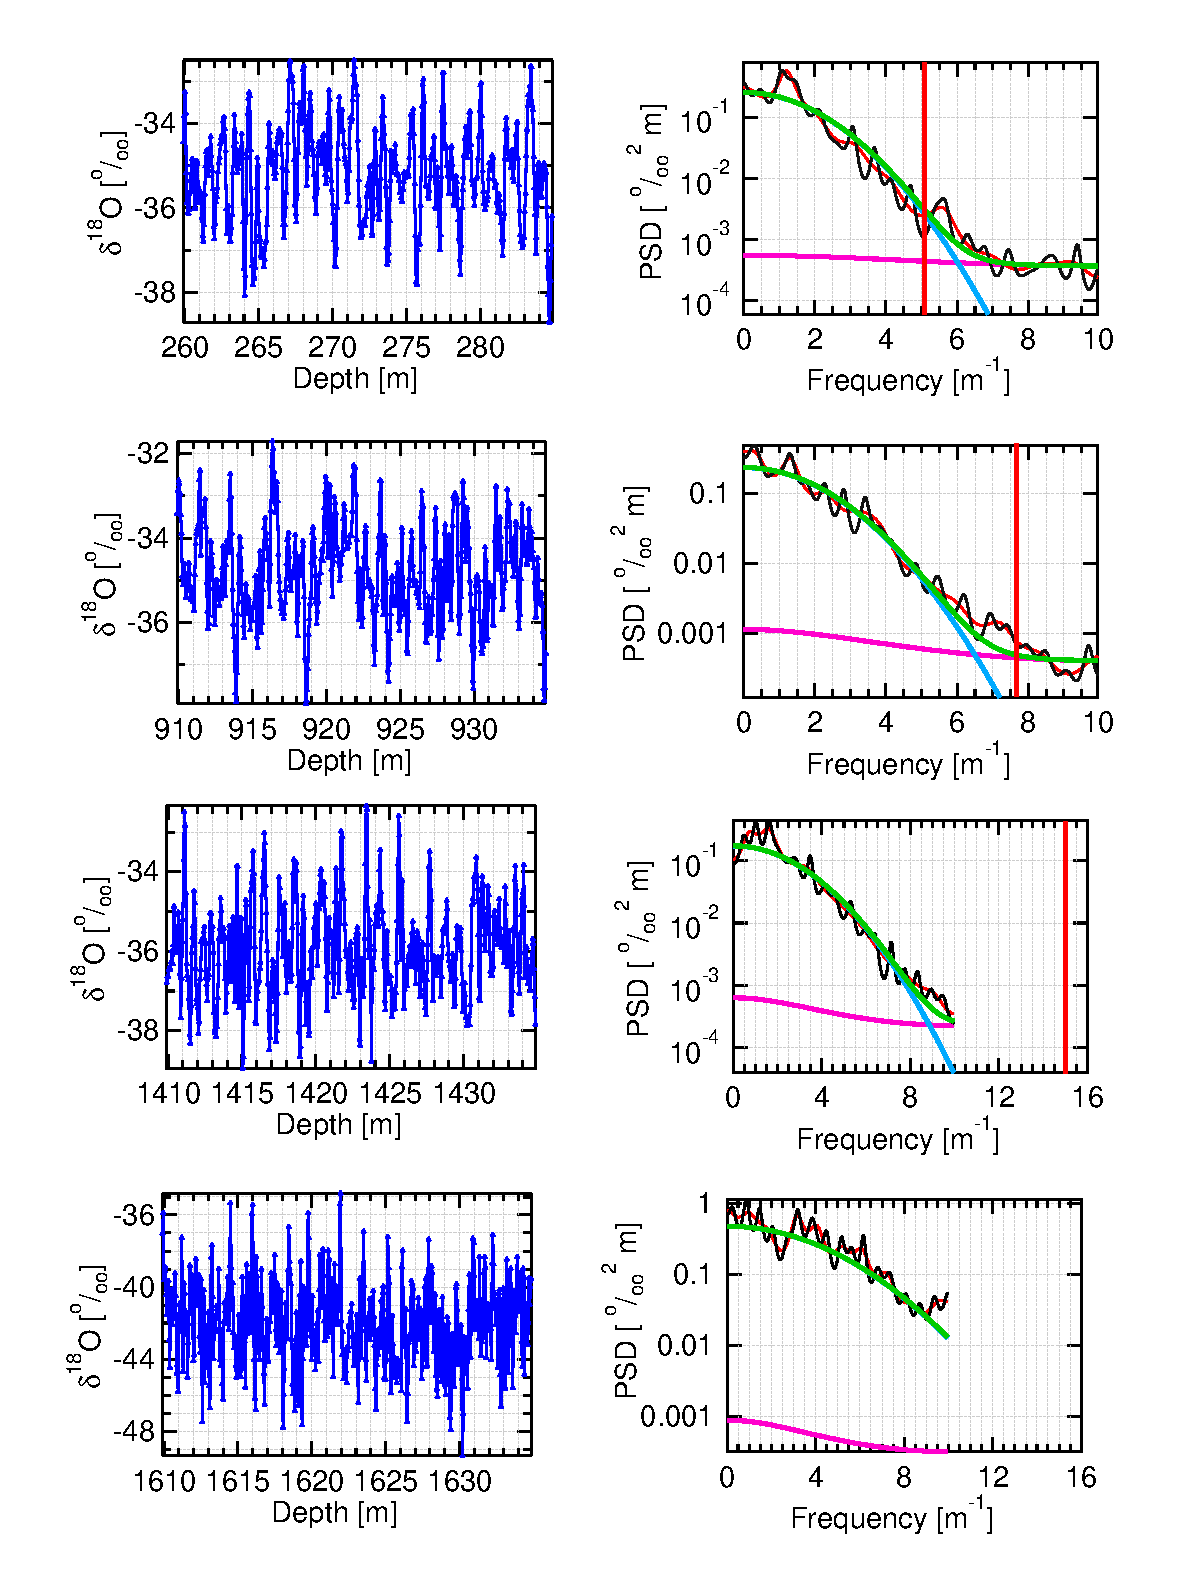
\includegraphics[width = 110mm]{spectral_estimate01}
\caption{Examples of raw \delOx data and estimated power spectral densities $\hat{P}_s$ for four different depth
intervals using $\mu = 30$ (red spectra) and $\mu = 40$ (black spectra). 
The power spectral model is illustrated; $P_s$ in green, $P_{\sigma}$ in cyan and 
${\vert \hat{\eta} \left( k \right) \vert} ^{2}$ in pink. The red vertical line in the top three plots
indicates the approximate position of the frequency representing the annual layer thickness. 
For the bottom plot this frequency is $\approx 40 \, \mathrm{m}^{-1}$ and omitted from the plot.}
\label{spectral01}
\end{figure}

\begin{figure*}
\vspace*{1mm}
\center
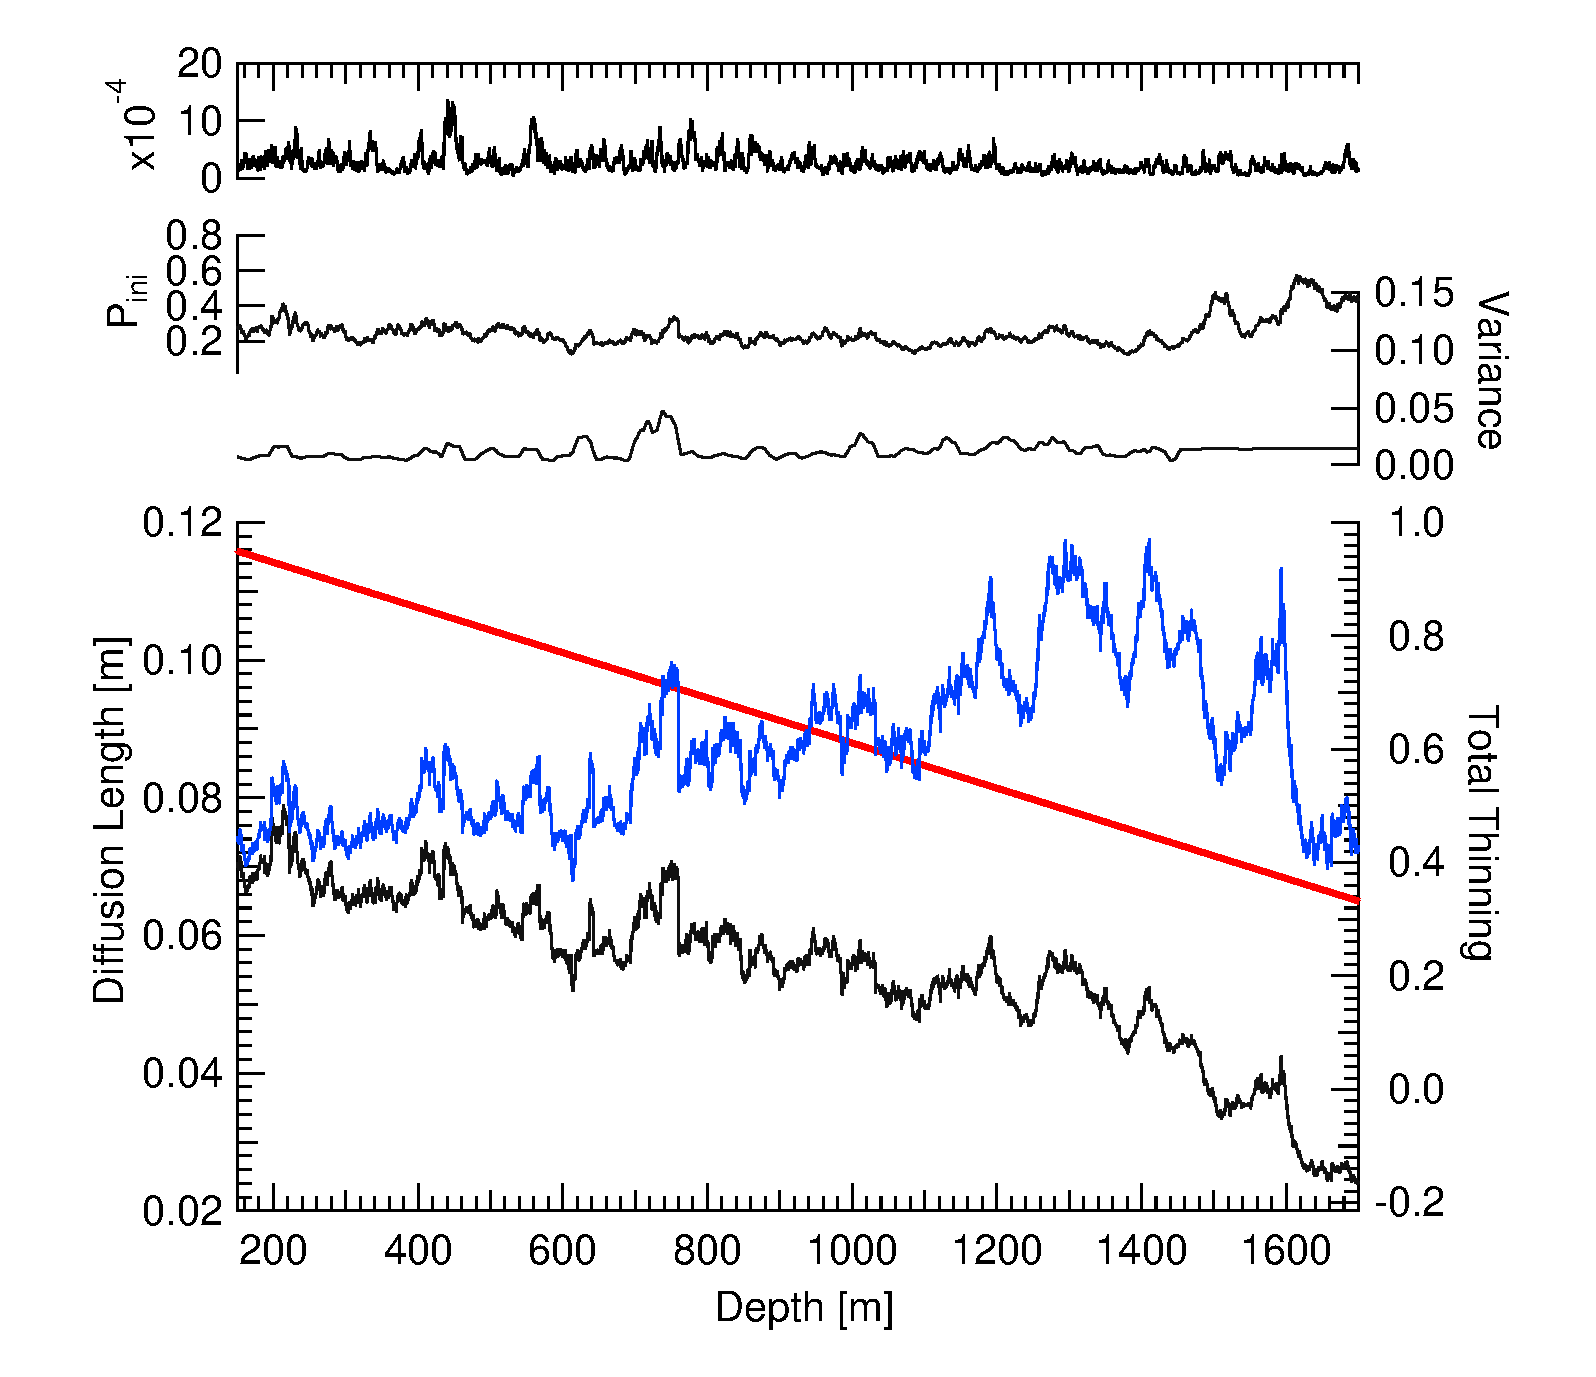
\includegraphics[width = 100mm]{spectral_estimate02}
\caption{Vertical profiles of $\sigma_{\mathrm{firn}}$, $S(z)\sigma_{\mathrm{firn}}$, $\sigma_{\mathrm{ice}}$ and $\sigma_i$
	For the calculation of 
	$\sigma_{\mathrm{firn}}$ the parameters we used for the H--L model were: 
	$P = 0.7$ Atm, $\rho_0 = 330 \mathrm{\;kgm^{-3}}$, 
	$\rho_{\mathrm{CO}} = 804.3 \;\mathrm{kgm^{-3}}$, $T = 242.15$ K, and 
	$A = 0.2 \;\mathrm{myr}^{-1}$ ice eq. 
	Top plot: Standard deviation
	of the 41 estimates of the diffusion length for every depth in m ice eq.}
\label{spectral02}
\end{figure*}

\begin{figure*}
\center
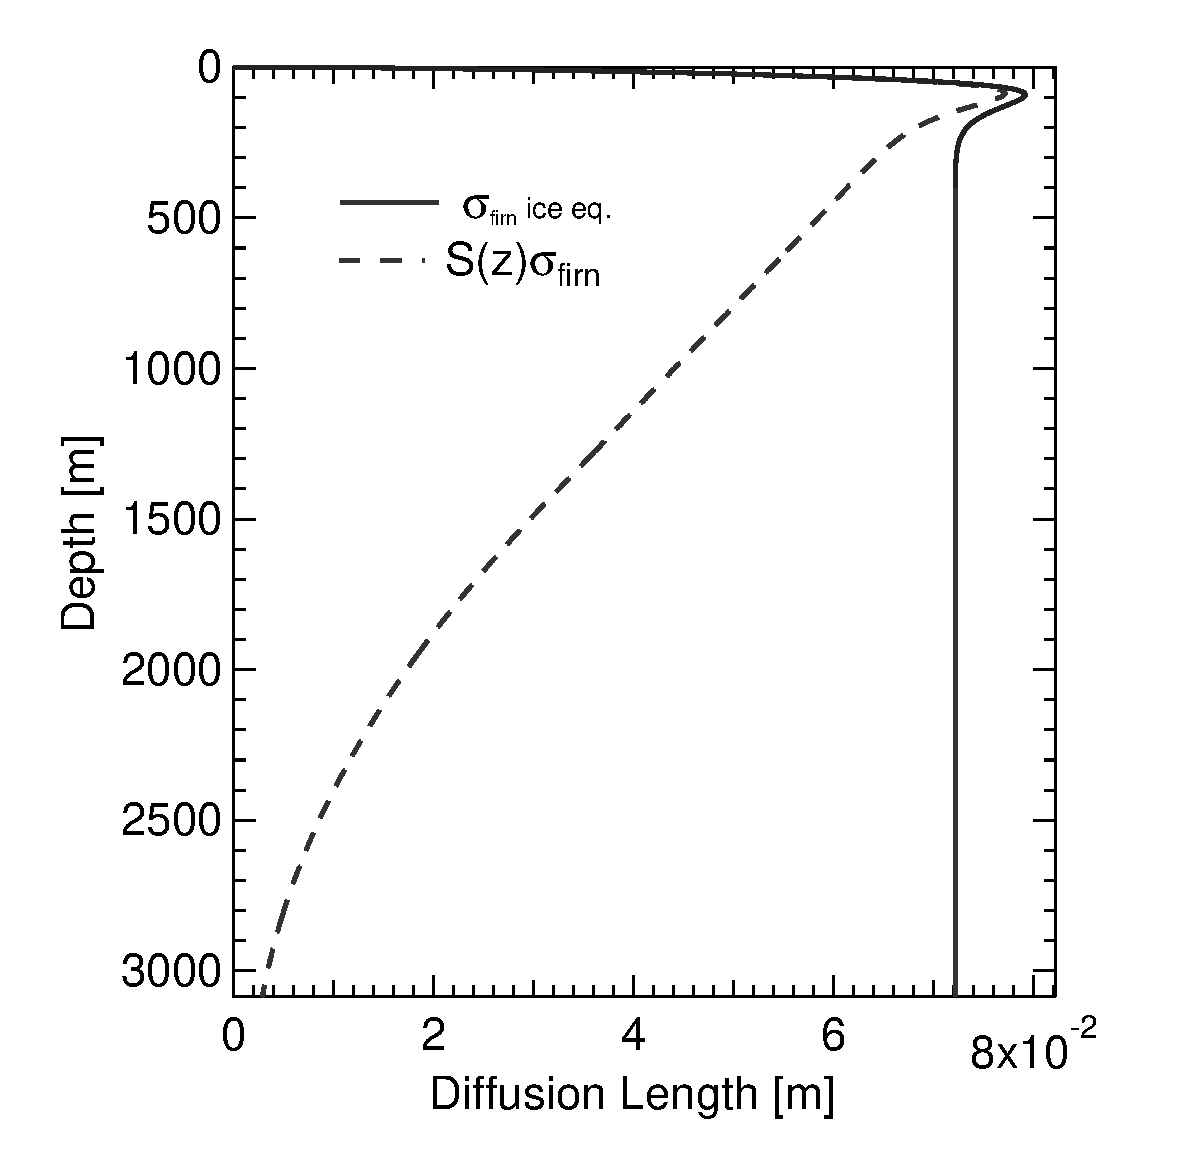
\includegraphics[width = 80mm]{spectral_estimate04}
\caption{Effect of the ice layer thinning on the value of the diffusion length.
	For the calculation of 
	$\sigma_{\mathrm{firn}}$ the parameters we used for the H--L model were typical of Holocene
	conditions for the NorthGRIP site: 
	$P = 0.7$ Atm, $\rho_0 = 330 \mathrm{\;kgm^{-3}}$, 
	$\rho_{\mathrm{CO}} = 804.3 \;\mathrm{kgm^{-3}}$, $T = 242.15$ K, and 
	$A = 0.2 \;\mathrm{myr}^{-1}$ ice eq. }
\label{spectral04}
\end{figure*}


\begin{figure*}
\center
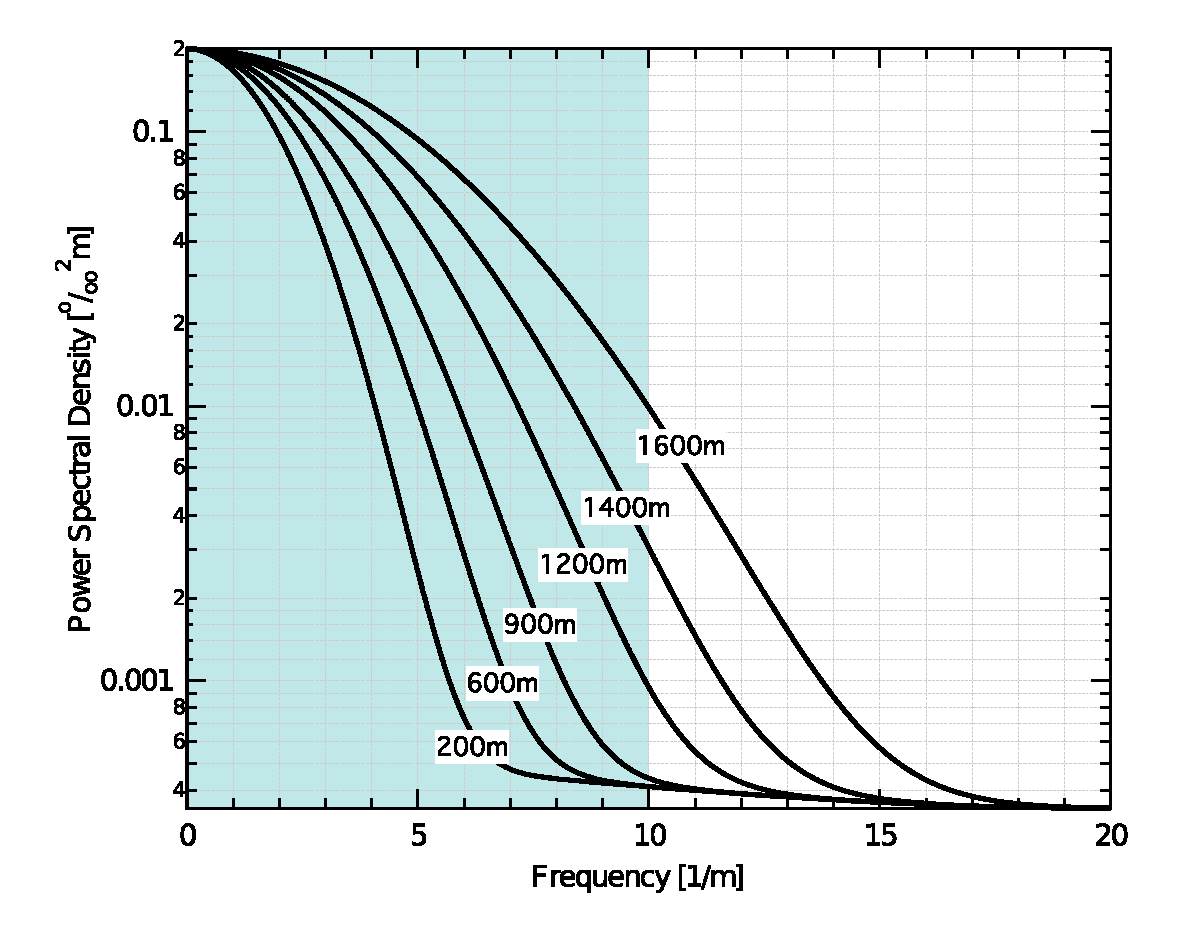
\includegraphics[width = 90mm]{spectral_estimate03}
\caption{Modeled power spectral densities for 6 different depths using diffusion length values from the 
calculation of Fig. \ref{spectral04} (Note that all plots represent identical accumulation
rate and temperature forcing at the surface). 
We use the spectral model as in Eq. \ref{powersd} with 
$q_1 = 0.15, P_{ini} = 0.2$. The highlighted area represents the expected spectra for the case of
$\Delta = 5 \mathrm{cm} \, \left(f_{Nyq} = 10 \, \mathrm{m}^{-1}\right)$ while the full range 
of the modeled spectra represents the case with 
$\Delta = 2.5\, \mathrm{cm} \, \left( f_{Nyq} = 20 \, \mathrm{m}^{-1} \right)$.}
\label{spectral03}
\end{figure*}

\begin{figure*}
\center
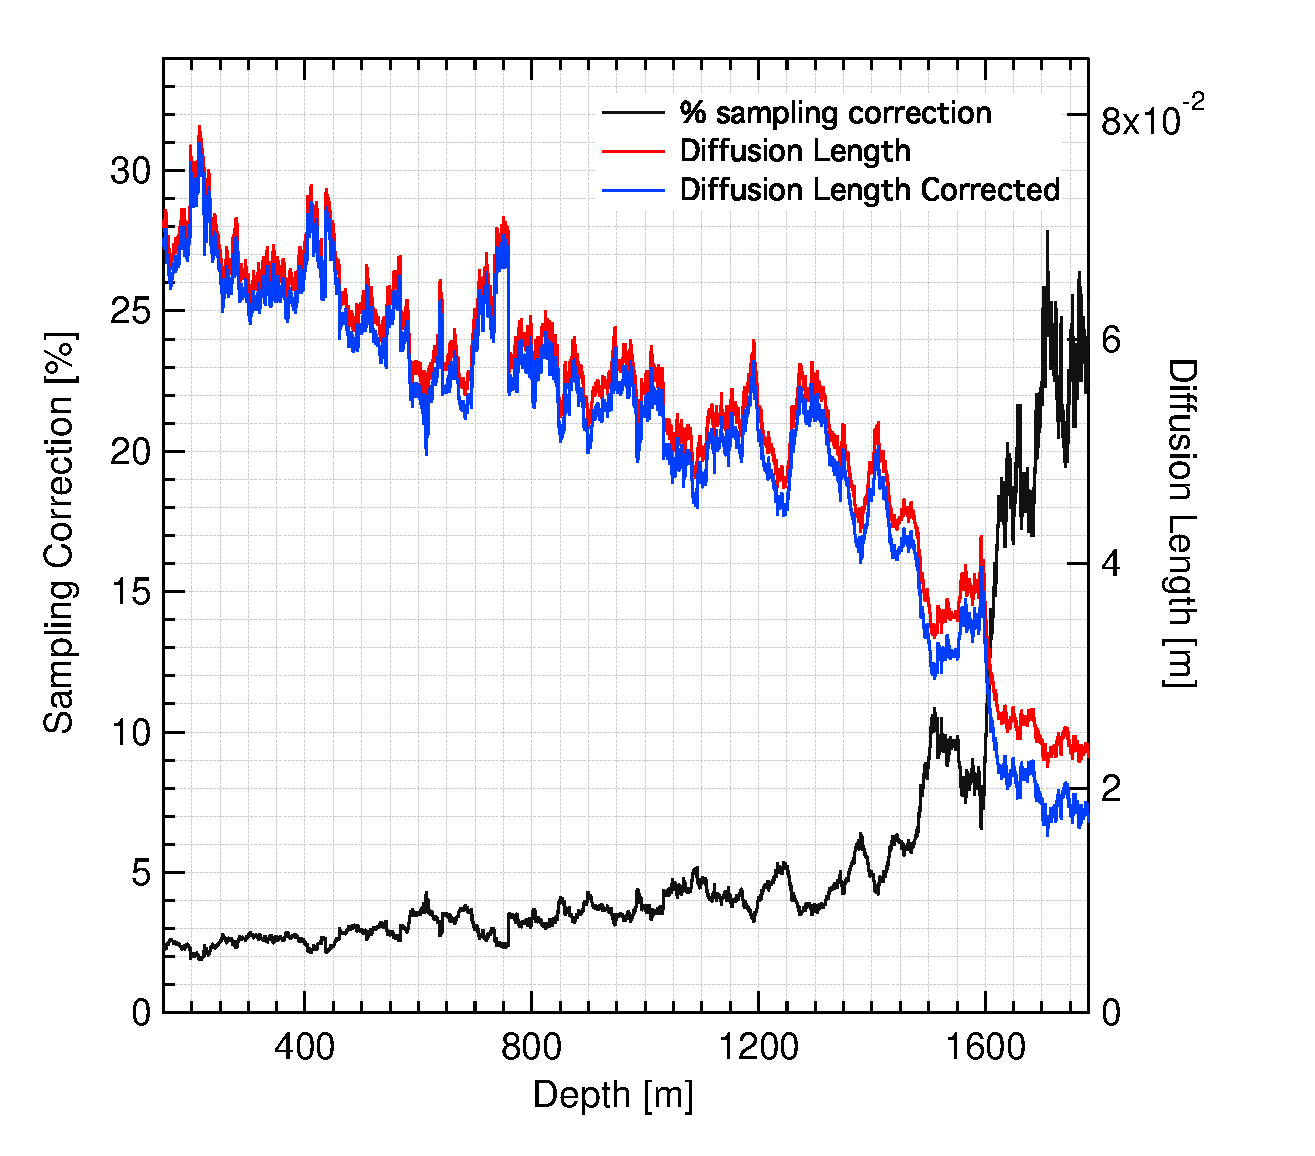
\includegraphics[width = 90mm]{discrete_sampling01}
\caption{Discrete sampling correction}
\label{discrete_sampling01}
\end{figure*}

\begin{figure*}
\center
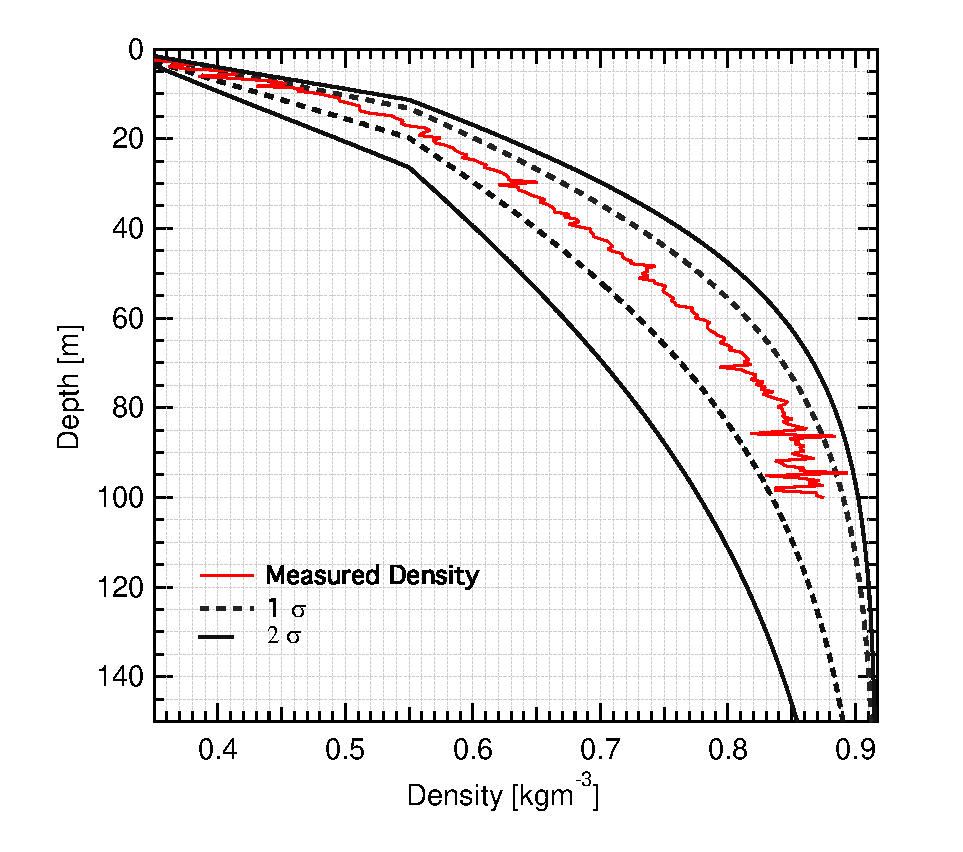
\includegraphics[width = 90mm]{density_NGRIP_fof1}
\caption{Firn density measurements from NorthGRIP (red) compared to implementations of 
the H-L densification model with varying values of $f$. Solid and dashed curves illustrate the 
range of $1\sigma$ and $2\sigma$ respectively.}
\label{density_NGRIP_fof1}
\end{figure*}



\begin{figure*}
\center
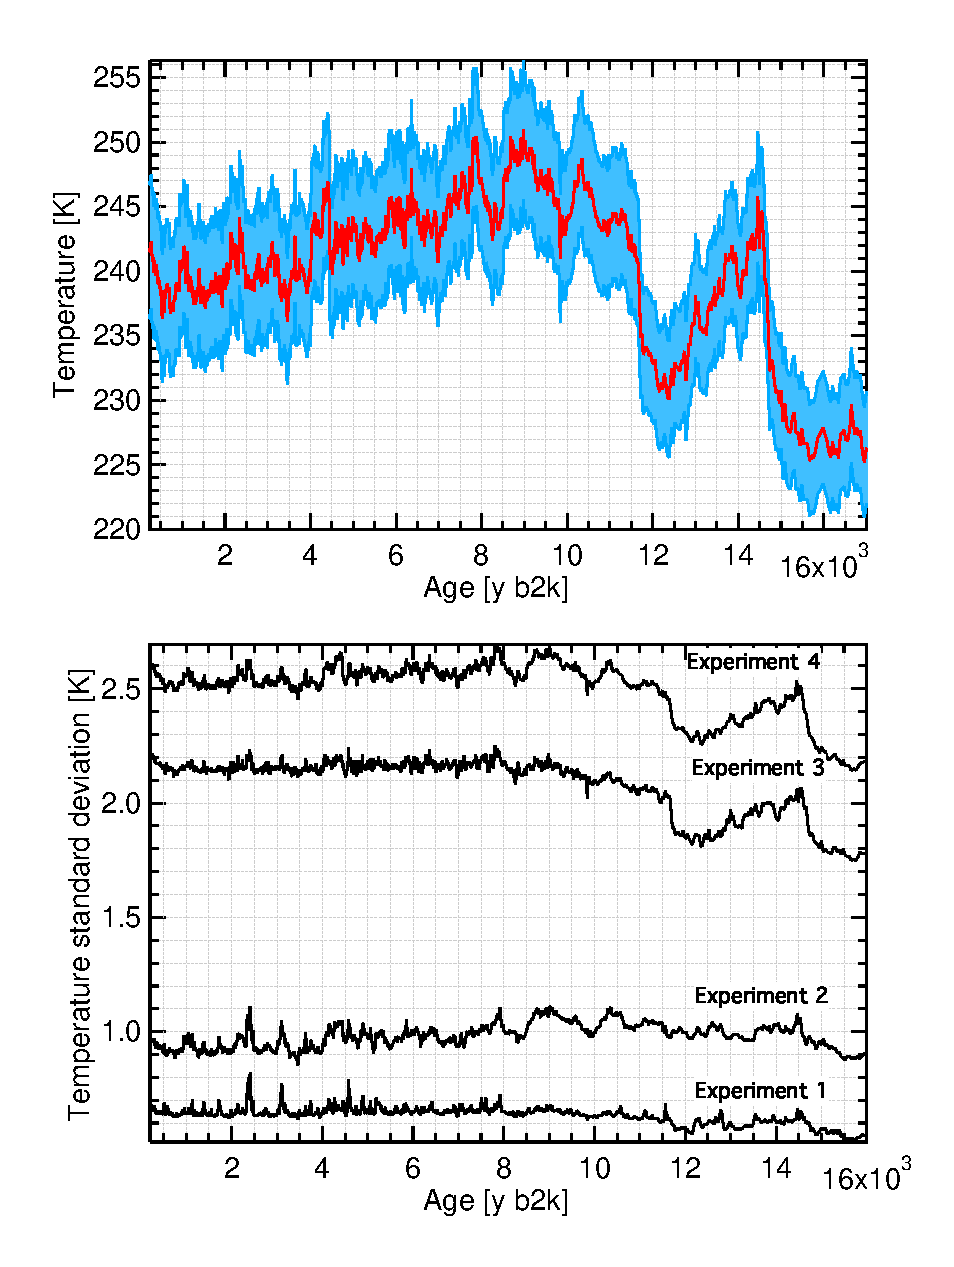
\includegraphics[width = 100mm]{mc_test_results}
\caption{Sensitivity tests results. The top panel illustrates the mean temperature history 
as calculated from Experiment 4 (all parameters varied) bracketed by the 95\% confidence interval estimated
with the sensitivity test. In the bottom panel we present the value of the standard deviation ($1\sigma$) 
for each sensitivity test.}
\label{mc_tests_results}
\end{figure*}

\begin{figure*}
\center
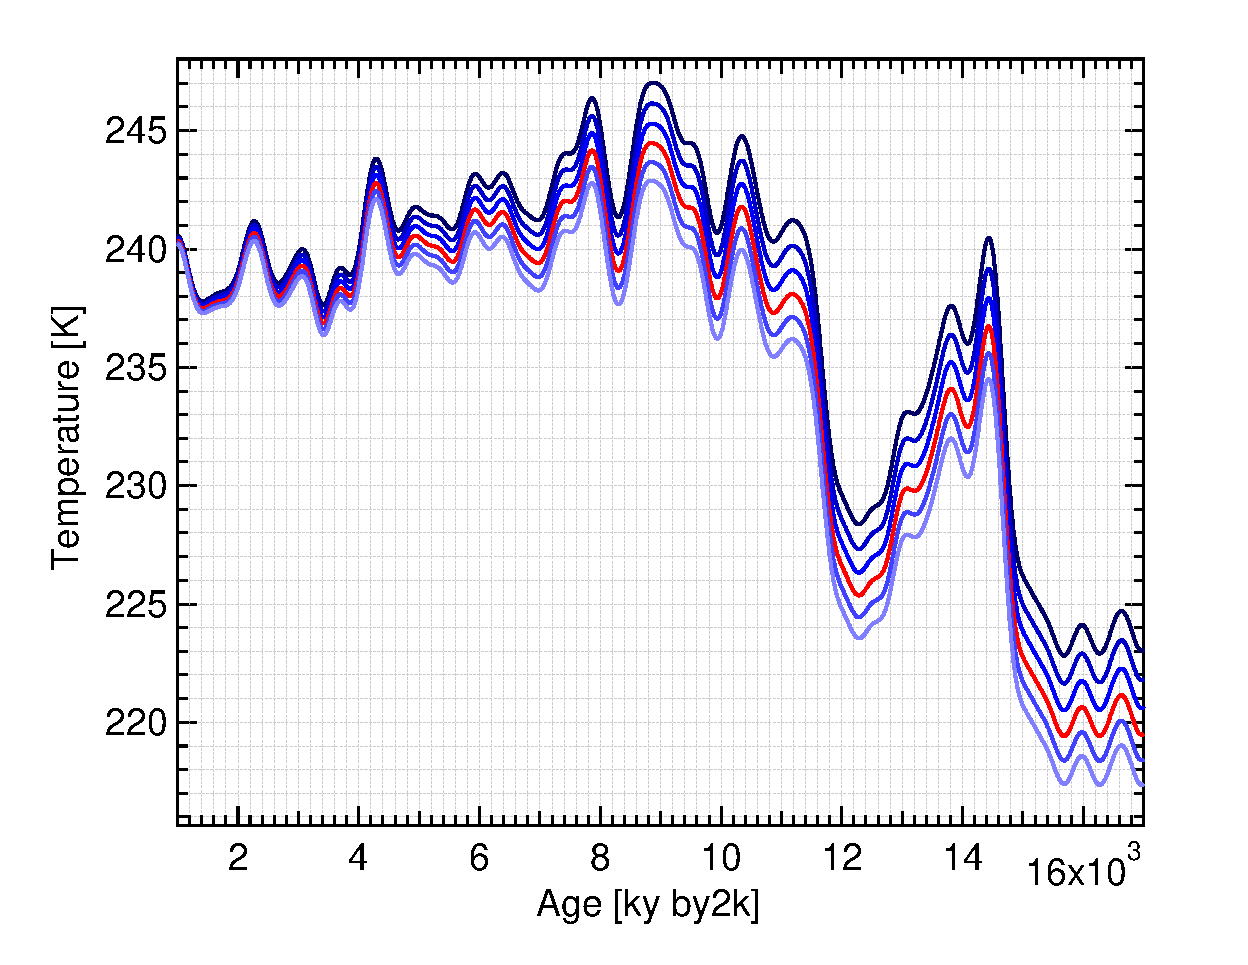
\includegraphics[width = 100mm]{./strain_uncertainty}
\caption{Ice thinning uncertainty illustrated. Temperature reconstructions 
for NorthGRIP using (from high to low) $S(2100m) = 0.22, 0.24, 0.26, 0.28, 0.30, 0.32$. 
Records filtered with a 500y low-pass filter.}
\label{strain_uncertainty}
\end{figure*}

\end{document}




\endinput
%%
%% End of file `elsarticle-template-harv.tex'.
